\documentclass{standalone}

\usepackage{tikz}
\usetikzlibrary{shapes, positioning, arrows.meta, calc, backgrounds, fit}

% states: (x,y)
\newcommand{\state}[2]{\node (#1#2) [rectangle, draw, font = \Large] at ($({1.5*(#2-#1)}, {2*(-#1-#2)})$) {$(#1, #2)$};}
% client/server/both transition from one state (x,y) to another (x',y')
\newcommand{\ctrans}[2]{\draw [ctrans] (#1.south west) -- (#2.north);}
\newcommand{\strans}[2]{\draw [strans] (#1.south east) -- (#2.north);}
\newcommand{\trans}[2]{\ctrans{#1}{#2} \strans{#1}{#2}}
\newcommand{\send}[2]{\draw [bend right, >=Stealth, ->] (#1) to (#2);}

\begin{document}
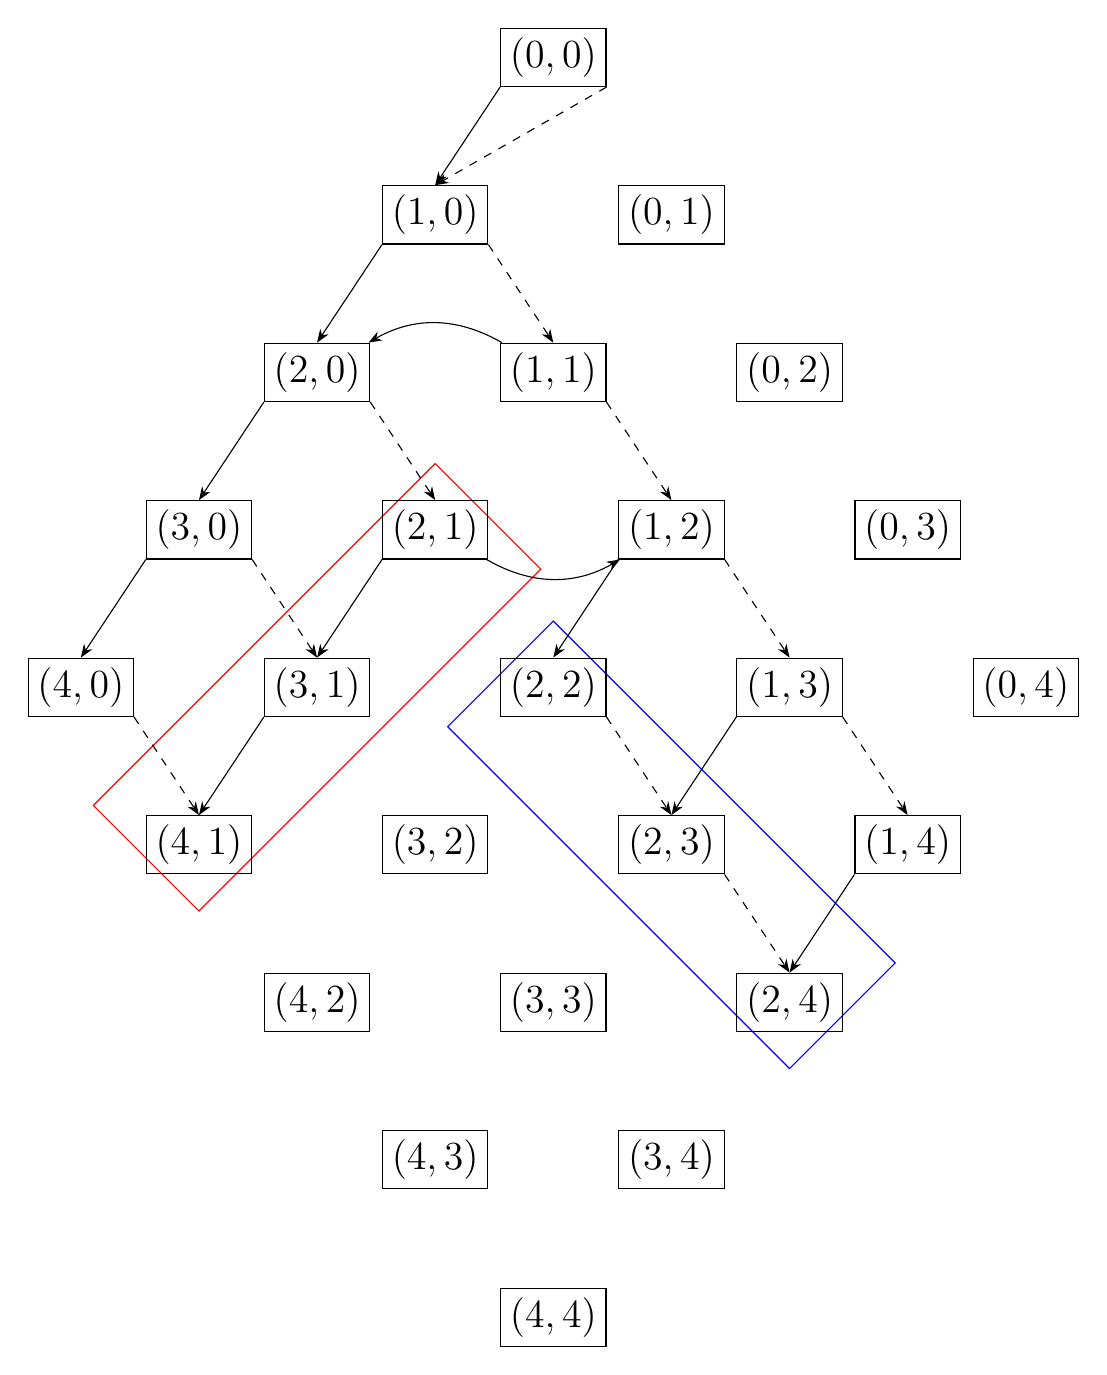
\begin{tikzpicture}[ctrans/.style = {>=Stealth, ->},
  strans/.style = {>=Stealth, ->, dashed}]
  \foreach \x in {0, 1, 2, 3, 4} {
	\foreach \y in {0, 1, 2, 3, 4} {
	  \state{\x}{\y}
	}
  }

  \trans{00}{10}

  \ctrans{10}{20}
  \ctrans{20}{30}
  \ctrans{30}{40}

  \strans{10}{11}
  \strans{11}{12}
  \strans{12}{13}
  \strans{13}{14}

  \send{11}{20}
  \strans{20}{21}
  \strans{30}{31}
  \strans{40}{41}
  \ctrans{21}{31}
  \ctrans{31}{41}
  
  \begin{pgfonlayer}{background}
	\node [draw, rectangle, red, rotate fit = 45, fit = (21) (31) (41)] {};
  \end{pgfonlayer}

  \send{21}{12}
  \ctrans{12}{22}
  \ctrans{13}{23}
  \ctrans{14}{24}
  \strans{22}{23}
  \strans{23}{24}

  \begin{pgfonlayer}{background}
	\node [draw, rectangle, blue, rotate fit = 45, fit = (22) (23) (24)] {};
  \end{pgfonlayer}
\end{tikzpicture}
\end{document}
